%%%%%%%%%%%%%%%%%%%%%%%%%%%%%%%%%%%%%%%%%%%%%%%%%%%%%%%%%%%%%%%%%%%%
%% I, the copyright holder of this work, release this work into the
%% public domain. This applies worldwide. In some countries this may
%% not be legally possible; if so: I grant anyone the right to use
%% this work for any purpose, without any conditions, unless such
%% conditions are required by law.
%%%%%%%%%%%%%%%%%%%%%%%%%%%%%%%%%%%%%%%%%%%%%%%%%%%%%%%%%%%%%%%%%%%%

\documentclass{beamer}
\usetheme[faculty=fi]{fibeamer}
\usepackage[utf8]{inputenc}
\usepackage[
  main=english, %% By using `czech` or `slovak` as the main locale
                %% instead of `english`, you can typeset the
                %% presentation in either Czech or Slovak,
                %% respectively.
  czech, slovak %% The additional keys allow foreign texts to be
]{babel}        %% typeset as follows:
%%
%%   \begin{otherlanguage}{czech}   ... \end{otherlanguage}
%%   \begin{otherlanguage}{slovak}  ... \end{otherlanguage}
%%
%% These macros specify information about the presentation
\title{A Neural Network-Evolutionary Computation framework for Remaining Useful Life Estimation} %% that will be typeset on the
\subtitle{David Laredo} %% title page.
\author{7 June, 2018}
%% These additional packages are used within the document:
\usepackage{ragged2e}  % `\justifying` text
\usepackage{booktabs}  % Tables
\usepackage{tabularx}
\usepackage{tikz}      % Diagrams
\usetikzlibrary{calc, shapes, backgrounds}
\usepackage{amsmath, amssymb}
\usepackage{url}       % `\url`s
\usepackage{listings}  % Code listings
\usepackage{hyperref}
\usepackage{verbatim}
%\usepackage{caption}
\usepackage{movie15}
\usepackage[labelsep=none]{caption}
\setbeamertemplate{caption}[numbered]

\frenchspacing
\captionsetup[figure]{labelformat=empty}


\begin{document}

  \frame{\maketitle}

  %\AtBeginSection[]{% Print an outline at the beginning of sections
    %\begin{frame}<beamer>
      %\frametitle{Outline for Section \thesection}
      %\tableofcontents[currentsection]
    %\end{frame}}

  \begin{darkframes}
    %\section{Dark Frames}
    
    \section{Introduction}
    
    \begin{frame}[label=introduction]{Introduction}
      %\framesubtitle{\TeX, \LaTeX, and Beamer}
      
	\begin{itemize}
		\item Maintenance of mechanical systems is, traditionally, carried out based on scheduling strategies.
		\begin{itemize}
			\item This strategies are costly and less capable of meeting the increasing demand of efficiency and reliability.
		\end{itemize}
		
		\item Intelligent Prognostics and Health Management (PMH) allow for maintenance based on the current health of the system.
		\item Here we define prognostics as the estimation of the remaining useful life (RUL) of a certain mechanical system.
	\end{itemize}      
      	
    \end{frame}
    
      \begin{frame}
      %\framesubtitle{}%     
      
      	\begin{itemize}
		\item RUL can be estimated based on history trajectory data (data driven).
		\begin{itemize}
			\item Model-based, data-driven and hybrid.
		\end{itemize}
		
		\item Here we present a framework for estimating the RUL of mechanical systems.
		
	\end{itemize}
         
    \end{frame}
    
    \begin{frame}
      %\framesubtitle{}%     
    
    The framework consists of an artificial neural network (ANN) as base regressor coupled with and evolutionary algorithm for fine tuning the data-related hyperparameters. \vspace{1em}
	
	The performance and reliability of the approach was tested using the CMAPS dataset. The results show that the proposed framework is competitive with the approaches shown in the current literature. 
      
    \end{frame}
      
    \begin{frame}{RUL of a commercial aircraft engine}
      %\framesubtitle{Test, validation and training sets}% 
      
      The CMAPS simulator is a NASA turbofan engine simulator that allows the user to specify different a number of operational settings and health parameters. 
      
      \begin{figure}[!htb]
		\begin{center}
			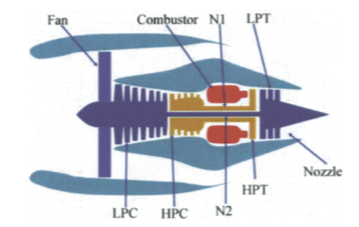
\includegraphics[width=70mm, height=50mm]{resources/cmaps_model.png}
			%\caption{The supervised learning process}
			\label{fig:cmaps}
		\end{center}
	\end{figure}
      
    \end{frame}
    
    \begin{frame}{RUL of a commercial aircraft engine}
      %\framesubtitle{Test, validation and training sets}% 
      
      The CMAPS dataset is a collection time-series where each element is a cycle for an specific engine settings.
      
      \begin{itemize}
      \item C-MAPS has 14 inputs (fuel flow and 13 health parameters).
      \item It can produce up to 58  outputs but for the avilable public dataset only 21 are published.
      \item The output is produced as time-series where each entry is an engine cycle.
      \item The goal is to estimate the number of cycles the engine can run before failure.
      \end{itemize}
      
    \end{frame}
    
     \begin{frame}{CMAPS dataset}
      %\framesubtitle{Test, validation and training sets}% 
      
      The CMAPS dataset is divided into 4 subsets
      
	\begin{table}[!htb]
	\centering
		\begin{tabular}{l | l l l l}
			\hline
		 	& \multicolumn{4}{c}{C-MAPSS}\\  
	 		Dataset & FD001 & FD002 & FD003 & FD004\\
  			\hline
  			Train Trajectories & 100 & 260 & 100 & 248\\
  			Test Trajectories & 100 & 259 & 100 & 248\\
  			Operating Conditions & 1 & 6 & 1 & 6\\
  			Fault Modes & 1 & 1 & 2 & 2\\
  			\hline
		\end{tabular}
	\caption{C-MAPSS Dataset details}
	\label{table:cmapss}
	\end{table}
      
    \end{frame}
    
    \begin{frame}{Performance metrics}
      %\framesubtitle{Test, validation and training sets}% 
      
      The performance of the proposed method is evaluated using the Root Mean Squared Error (RMSE) and the RHS score defined as:

	\begin{align}
	s &= \frac{1}{N} \sum_{i=1}^{N}{s_i} \nonumber \\
	s_i &= \begin{cases} 
      e^{-\frac{d_i}{13}} - 1 & d_i < 0, \\
      e^{\frac{d_i}{10}} - 1 & d_i \geq 0
	\end{cases}
	\label{eq:rhs}
	\end{align}
      
	where $d_i = RUL_i^p - RUL_i$.      
      
    \end{frame}
    
	\begin{frame}{Data pre-processing}
      %\framesubtitle{Test, validation and training sets}% 
      
      The following steps are applied to the data before being processed by the regressor

	 \begin{itemize}
	  \item Data is gropued into time-windows of size $n_w$ and stride $n_s$.
	  \item A piecewise linear degradation model is used for the RUL of the engines.
	  \begin{itemize}
	  	\item $R_e$ is used as the upper limit for the piecewise linear degradation model.
	  \end{itemize}
	  \item The data is standardized using min-max method to make the data be in the range (-1, 1).
	  \item For the test set a time window is generated from the last $n_w$ data instances.
	\end{itemize}	       
      
    \end{frame} 
    
    \begin{frame}{Estimating RUL using ANN as regressor}
      %\framesubtitle{Test, validation and training sets}% 
      
	The chosen ANN architecture complies with the following parameters    
      
	\begin{itemize}
	\item It was chosen among 6 different architectures.
	\item Two objectives were pursued, that the architecture was compact and efficient.
	\item FD001 was used for evaluating the performance of the regressor.
	\item The chosen architecture must have a good compromise between the scores and its size.
	\item Each architecture was run 10 times and their results were averaged.
	\end{itemize}	      
     
     \end{frame}
     
     \begin{frame}
     
	The chosen architecture is     
     
     \begin{table}[!htb]
	\centering
		\begin{tabular}{l l l l}
		\hline
		Layer & Shape & Activation & Additional Information\\
  		\hline
  		Fully connected & 30 & ReLU & L2-$\lambda = 0.2$\\
  		Fully connected & 10 & ReLU & L2-$\lambda = 0.2$\\
  		Fully connected & 1 & Linear & \\
  		\hline
	\end{tabular}
	\caption{Proposed Neural Network architecture}
	%\caption{}
	\label{table:proposed_nn}
	\end{table}
	
	and its scores for dataset FD001 are
	
	\begin{table}[!htb]
	\centering
	\begin{tabular}{l | r | r}
	\hline	
	Tested Architecture & Avg. RMSE  & Avg. RHS \\
  	\hline
  	Chosen & 18.31 & 10.76\\
  	\hline
	\end{tabular}
	\caption{Average results for chosen architecture}
	\label{table:tested_architectures_100}
	\end{table}
      
    \end{frame}
    
    \begin{frame}{Choosing the optimal data-related parameters}
      %\framesubtitle{Test, validation and training sets}% 
      
	The performance of the regressor can be improved by choosing the appropriate set of data-related parameters. Here we make use of evolutionary algorithms to pick the best possible choice of such parameters. \vspace{1em}
	
	 Let $\mathbf{v} = (n_w, n_s, R_e)$, where $n_w \in \left[1, b\right]$, $n_s \in \left[1, 10\right]$ and $R_e \in \left[90, 120 \right]$ and all the intervals are integer intervals. The value of $b$ is dependent upon the specific subset.      
     
     \end{frame}
     
     \begin{frame}
      %\framesubtitle{Test, validation and training sets}% 
     
     The task is now to pick $\mathbf{v}$ such that the RMSE for each subset, and using the architecture defined in Table \ref{table:proposed_nn}, is minimized. \vspace{1em}.
     
     For this end Differential Evolution was used, the following rules were followed for the optimization process:
     
     \begin{itemize}
     \item A population of 30 elements was run for 20 generations.
     \item The values of the components of $\mathbf{v}$ were rounded to the nearest integer at each iteration.
     \item The Neural Network wasn't trained for the entire 100 epochs but for 20 instead.
     \item best1bin strategy was used for crossover and elitism.
     \item Maximum allowable window sizes were used for each dataset.
     \end{itemize}
     
     \end{frame}
     
          \begin{frame}
      %\framesubtitle{Test, validation and training sets}% 
     
     Since subsets FD001/FD003 and FD002/FD004 are similar in the number of fault modes the optimization process was only run for subsets FD001 and FD002 and the results obtained were applied to FD003 and FD004. Table ... displays the obtained values for $\mathbf{v}$. \vspace{1em}
     
     \begin{table}[!htb]
\centering
\begin{tabular}{l l l l l}
	\hline
	 Dataset & $n_w$ &$n_s$ & $R_e$\\
  	\hline
  	FD001 & 30 & 2 & 120\\
  	FD002 & 20 & 2 & 120\\
  	FD003 & 30 & 2 & 120\\
  	FD004 & 18 & 2 & 120\\
  	\hline
\end{tabular}
\caption{Data-related parameters for each subset as obtained by DE.}
\label{table:data_params_de}
\end{table}
     
     \end{frame}
     
     \begin{frame}
      %\framesubtitle{Test, validation and training sets}% 
     
     The average results over 10 trials obtained by training the network using the parameters shown in Table \ref{table:data_params_de} are displayed in Table \ref{table:results_ann_de}. \vspace{1em}
   
\begin{table}[!htb]
\centering  
\begin{tabular}{l | r r r | r r r}
	\hline	
	& \multicolumn{3}{| c}{RMSE} & \multicolumn{3}{| c}{RHS} \\
	Data Subset & Min. & Max. & Avg. & Min. & Max. & Avg. \\
  	\hline
  	FD001 & 14.78 & 15.25 & 14.90 & 3.41 & 4.40 & 3.94 \\
  	FD002 & 29.76 & 31.55 & 30.67 & 59.25 & 95.36 & 69.25\\
  	FD003 & 15.05 & 16.05 & 15.54 & 3.24 & 4.98 & 3.86\\
  	FD004 & 34.61 & 37.75 & 35.58 & 55.46 & 91.94 & 69.06\\
  	\hline
\end{tabular}

\caption{Scores for each dataset using the data-related parameters obtained by DE.}
\label{table:results_ann_de}
\end{table}
     
     \end{frame}
     
\begin{frame}{Comparison with state-of-the-art}
      %\framesubtitle{Test, validation and training sets}% 
     
     The proposed method is compared with some of the state-of-the-art methods proposed for this dataset. Only FD001 is used for comparison as it is the subset whose results are consistently reported in the majority of the approaches compared.
   
\begin{table}[!htb]
\centering
\begin{tabular}{l r}
	\hline	
	Method & RMSE \\
  	\hline
  	ESN-Kalman \cite{Peng2012} & 63.45\\
  	SVM Classifier \cite{Louen2013}  & 29.82\\
  	Time Window ANN \cite{Lim2016} & 15.16\\
  	Multi-objective Networks Ensemble \cite{Zhang2016} & 15.04\\
  	Deep CNN \cite{Babu2016} & 18.45\\
  	\textbf{Proposed method} & 14.90\\
  	\hline
\end{tabular}
\caption{Performance comparisons of the proposed method.}
\label{table:results_comparison}
\end{table}
     
     \end{frame}
     
\begin{frame}{Conclusions}
      %\framesubtitle{Test, validation and training sets}% 
     
	Here we presented a method for estimating the RUL of jet-engines, the highlights of the presented method are:     
     
	\begin{itemize}
	\item A systematic method for estimating the RUL of mechanical components was presented.
	\item The proposed method is competitive against other state-of-the-art methods in terms performance indicators.
	\item The chosen ANN architecture is lightweight.
	\item The presented methodology is, in theory, applicable to other mechanical systems with little to no change.
	\end{itemize}
     
     \end{frame}
     
     \section{Citations_and_Bibliography}

\begin{frame}[allowframebreaks]
        \frametitle{References}
        \bibliographystyle{amsalpha}
        \bibliography{reference_rul_paper.bib}
\end{frame}
    
    %\end{comment}

  \end{darkframes}
\end{document}
